% A single, figure-led slide on density-matrix prediction.
% Compile:  pdflatex density_matrix_prediction.tex   (needs fig/*.pdf)
% Figures are regenerated by fig/make_figs.py from runs 121/122 on df_db_mp2.
\documentclass[aspectratio=169,11pt]{beamer}
\usetheme{default}
\usepackage{graphicx}
\usepackage{amsmath}
\setbeamertemplate{navigation symbols}{}
\setbeamercolor{structure}{fg=black!75}
\setbeamerfont{frametitle}{size=\large,series=\bfseries}
\definecolor{fnloss}{HTML}{2B7A4B}
\definecolor{mseloss}{HTML}{B03A3A}

\begin{document}

\begin{frame}{Predicting the one-particle density matrix}

\centering

%% ---- what the 1-RDM is, and how it is represented -----------------------
\vspace{-2pt}
{\footnotesize
\[
  \gamma(r,r')
  \;=\; N\!\!\int\!\Psi^{*}(r,x_2\ldots x_N)\,\Psi(r',x_2\ldots x_N)\,
        \mathrm{d}x_2\cdots\mathrm{d}x_N
  \;=\; \sum_{\mu\nu} D_{\mu\nu}\,\phi_\mu(r)\,\phi_\nu(r')
\]}

\vspace{-10pt}
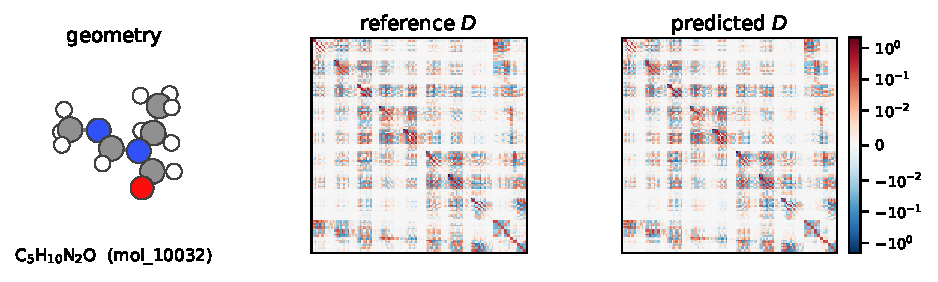
\includegraphics[width=0.68\textwidth]{fig/pipeline.pdf}

\vspace{-2pt}
{\footnotesize\itshape
15\,000 QM9 molecules, 6\text{-}31G*, MP2 \quad$\cdot$\quad 750 held out}

\vspace{1pt}
\hrule
\vspace{1pt}

%% ---- how it is trained, and what that buys ------------------------------
\begin{columns}[c]
\begin{column}{0.345\textwidth}
\centering\scriptsize
\[
  \textcolor{mseloss}{
    \mathcal{L} = \lVert\Delta D\rVert_F^{2}
    = \textstyle\sum_{\mu\nu}\Delta D_{\mu\nu}^{2}}
\]
\vspace{-9pt}
\[
  \textcolor{fnloss}{
    \mathcal{L} = \iint\!\big[\gamma-\tilde\gamma\big]^{2}
    = \operatorname{tr}\!\big(\Delta D\,S\,\Delta D\,S\big)}
\]
\end{column}
\begin{column}{0.645\textwidth}
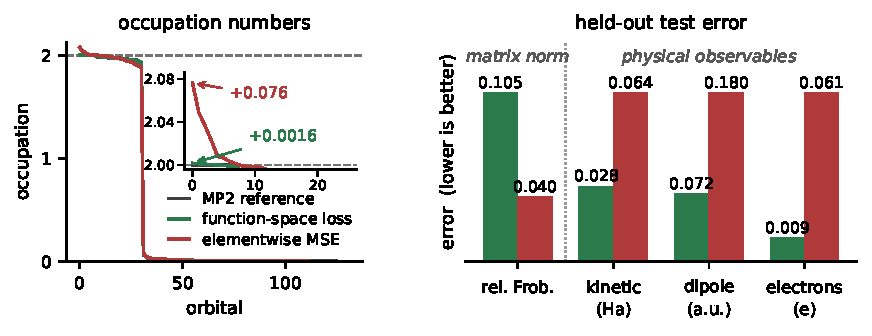
\includegraphics[width=0.97\textwidth]{fig/results.pdf}
\end{column}
\end{columns}

\end{frame}

\end{document}
